
\documentclass[a4paper, 12pt]{article}
\usepackage{geometry}
\geometry{margin=2cm}
\usepackage{graphicx} % Required for the inclusion of images
\usepackage[utf8]{inputenc}
%\usepackage{natbib} % Required to change bibliography style to APA
\usepackage{amsmath} % Required for some math elements 
\usepackage[spanish]{babel} 
%\usepackage{fontspec}
\usepackage{lineno,hyperref}
\usepackage{upgreek}
\usepackage{gensymb}
\usepackage{textcomp}
\usepackage{amssymb}
\usepackage{textgreek}
\usepackage{float}
\usepackage{fancyhdr}
\usepackage{dirtytalk}

\allowdisplaybreaks
%\textwidth18cm
%\textheight22cm
%\topmargin0cm
%\oddsidemargin2cm
%\hypersetup{hidelinks}

\usepackage{multirow}

\hypersetup{
    colorlinks=true,
    linkcolor=blue,
    }
\graphicspath{{img}}
\setlength\parindent{0pt} % Removes all indentation from paragraphs

\renewcommand{\labelenumi}{\alph{enumi}.} % Make numbering in the enumerate environment by letter rather than number (e.g. section 6)

\renewcommand{\b}{\textbf}

\newsavebox{\mygraphic}
\sbox{\mygraphic}{
\includegraphics[height=1cm]{logoUNRN.jpg}}


\pagestyle{fancy}

\fancyhead{}

\headheight 16pt

\fancyhead[LO]{\setlength{\unitlength}{1in}
	\begin{picture}(0,0)
		\put(0,0){\usebox{\mygraphic}}
	\end{picture}
	\hspace{1cm}
}

\fancyhead[CO] {\hspace{1.5cm} \large Física I: Ingenierías Ambiental, Electrónica y Telecomunicaciones}

%esto me pareció piola para enumerar los ejercicios
%lo saqué de acá: https://tex.stackexchange.com/questions/302948/numbered-exercises-as-sections
%%%%%%%%%%%%%%%%%%%%%%%%%%%%%%%%%%%%%%%%%5
\newcounter{eje}
\setcounter{eje}{0}
\newcounter{subeje}
\setcounter{subeje}{-1}
\renewcommand\thesubeje{\arabic{eje}\alph{subeje}}%
\newcommand \eje{%
  \vspace{.2cm}
  \par\noindent
  \ifnum\value{subeje}>-1
    \refstepcounter{subeje}%
    \llap{\thesubeje)\quad}%
  \else
    \refstepcounter{eje}%
    \llap{\theeje)\quad}%
  \fi
}
\begin{document}
\pagestyle{fancy}

\begin{center}

	{\Large \textbf{Práctica 2b}}
 
\vspace{.2cm}

{Dinámica}
\end{center}

\eje  [4.3] Un objeto de 4.0 kg tiene una velocidad de 3.0 m/s \b i en determinado instante. Ocho
segundos después, su velocidad es de 8.0 m/s \b i + 10.0 m/s \b j. Asumiendo que el objeto estaba sujeto a una fuerza neta constante, encuentre las componentes de la fuerza y su magnitud.

\eje [4.4] Cinco fuerzas tiran de una caja de 4.0 kg como se muestra en la figura adjunta. Encuentre la
aceleración de la caja y exprésela:

a) en notación vectorial;

b) brindando su magnitud y dirección.
\begin{figure}[H]
\begin{center}
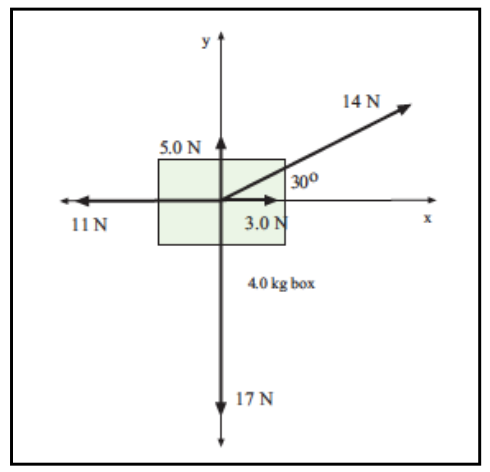
\includegraphics[clip,width = .45\columnwidth]{2bf2}
\end{center}
\end{figure}

\eje [p.31] Calcular la aceleración de las manzanas y la tensión en la soga para el sistema de la figura
(sí, las manzanas tienen esas masas, Newton no era sólo bueno con la mecánica, sino también
tenía un don para cultivar manzanas; ah, considere que no hay rozamiento).
\begin{figure}[H]
\begin{center}
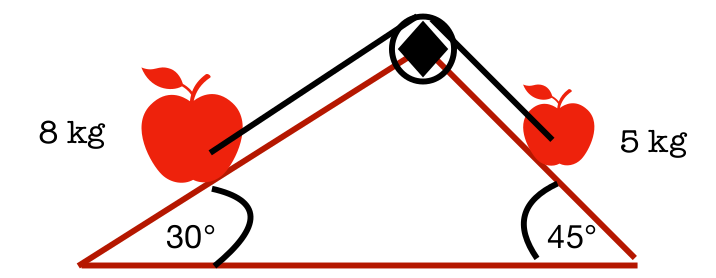
\includegraphics[clip,width = .45\columnwidth]{2bf3}
\end{center}
\end{figure}

\eje [p.35] Tenemos el sistema de la figura adjunta, donde la manzana con masa m$_1$ = 6 kg y la manzana con
masa m$_3$ = 3 kg, están inicialmente en reposo. Se las suelta y se verifica que la manzana con masa
m$_1$ tarda 2 s en tocar el piso. Calcular:

a) la aceleración de la manzana con masa m$_2$ durante el movimiento (está pegada a la m$_3$);

b) el valor de m$_2$ y

c) la fuerza de contacto entre las manzanas con masas m$_2$ y m$_3$ durante el movimiento.
\begin{figure}[H]
\begin{center}
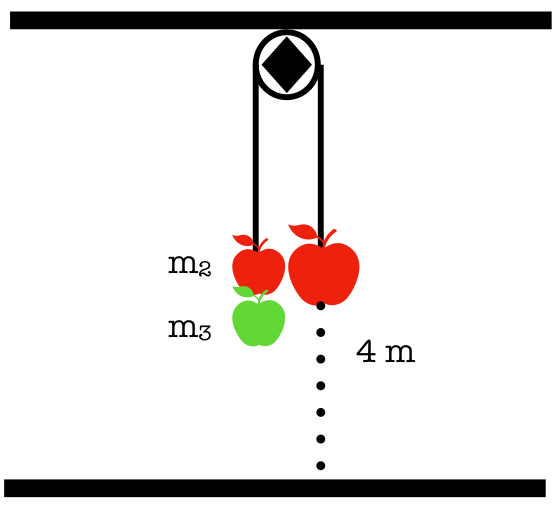
\includegraphics[clip,width = .45\columnwidth]{2bf4}
\end{center}
\end{figure}

\eje [p.37] El viejito de Newton está parado sobre una balanza, pero porque se ha vuelto un pillo, la balanza la colocó dentro de un montacargas. Si la balanza le marca una medida menor que su
peso real (por eso lo pillo), entonces el montacargas:

a) sube a velocidad constante;

b) baja a velocidad constante;

c) asciende acelerando;

d) se encuentra en reposo;

e) desciende acelerando;

f) desciende frenando.

\eje [p.42] Dos manzanas de masas m$_1$ = 9 kg y m$_2$ = 3 kg se encuentran inicialmente en reposo y se
hallan unidas por una soga y una polea ideales como muestra la figura:

a) calcule la aceleración de la manzana con masa m$_2$ si se desprecia todo tipo de rozamiento;

b) si se intercambian las manzanas entre sí, ¿cuál será la aceleración de la manzana m$_1$?
\begin{figure}[H]
\begin{center}
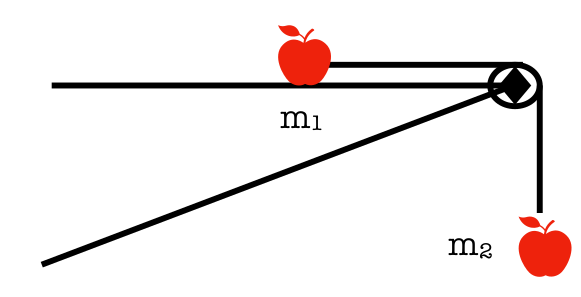
\includegraphics[clip,width = .45\columnwidth]{2bf6}
\end{center}
\end{figure}

\eje [p.55] Una manzana de 5 kg se mueve con velocidad de 10 m/s por una pista horizontal y recta
de Scalextric sin rozamiento (claramente adaptada para manzanas, la jubilación al viejito de
Newton no le alcanza para un “Sebring 1964”, entonces se las arregla con manzanas). Después,
la manzana entra en una zona con rozamiento. Calcular:

a) la aceleración que tiene la manzana “Sebring 1964” mientras se va frenando en la zona con
rozamiento (considere $\mu_e$ = 0,5 ; $\mu_d$ = 0,3);

b) la fuerza de rozamiento estático una vez que se detuvo;

c) la fuerza mínima que hay que ejercer para volver a poner la manzana en movimiento.

\eje [p.61] Después de ahorrar tres jubilaciones producto de su trabajo como Director de la Moneda,
allá por el 1700, el viejito de Newton pudo finalmente comprarse el Sebring 1964 que tanto quería
(claro, escala 1/24). Lo puso a andar a 20 m/s y luego lo hizo frenar hasta detenerlo (considere
$\mu_e$ = 0.8 ; $\mu_d$ = 0.4). Calcule, entonces, la distancia de frenado si el viejito de Newton:

a) le bloquea las ruedas,

b) no le bloquea las ruedas al Sebring 1964.

\eje [p.73] Para el sistema de la figura, describa la evolución de las (súper)manzanas y calcule la aceleración en los siguientes casos (considere $\mu_e$ = 0.8 ; $\mu_d$ = 0.4):

a) se libera el arreglo a partir del reposo;

b) se lo impulsa imprimiendo una velocidad inicial a la (súper)manzana “A” hacia abajo.
\begin{figure}[H]
\begin{center}
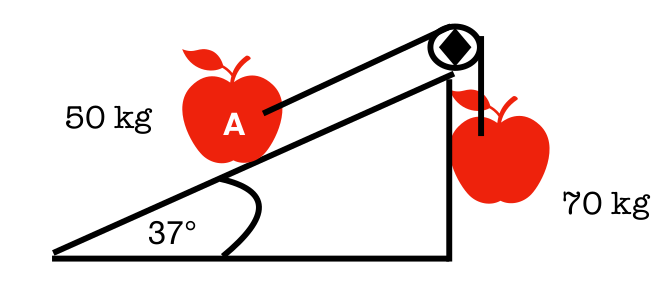
\includegraphics[clip,width = .45\columnwidth]{2bf9}
\end{center}
\end{figure}

\eje [p.77] Se tiene el sistema de la figura, en el cual la masa de las manzanas es de m$_1$ = 3 kg, m$_2$ = 3
kg y m$_3$ = 1 kg. Si bien entre las manzanas con masas m$_1$ y m$_2$ hay rozamiento (considere $\mu_e$ = 0.8 ; $\mu_d$ = 0.2), no lo hay entre la manzana con masa m$_2$ y la superficie sobre la que está
apoyada, ni entre sogas y poleas, dado que son ideales.

a) Sabiendo que las manzanas con masas m$_1$ y m$_2$ no deslizan una respecto de la otra, calcule la
fuerza de rozamiento entre ellas;

b) calcule cuál sería el máximo valor de la manzana con masa m$_3$ para que las manzanas con
masas m$_1$ y m$_2$ se muevan juntas.
\begin{figure}[H]
\begin{center}
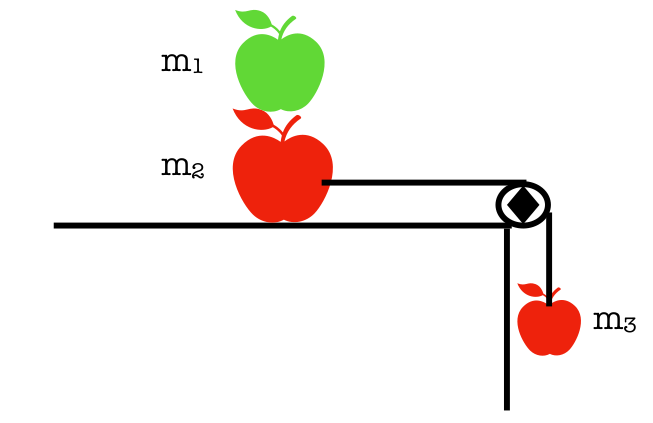
\includegraphics[clip,width = .45\columnwidth]{2bf10}
\end{center}
\end{figure}

\eje [p.91] Se cuelga una manzana de 2 kg de un resorte (k = 2 N/cm) y se la coloca en un ascensor
(sí, el viejito de Newton estaba aburrido). Calcule el estiramiento del resorte en los siguientes
casos:

a) ascensor quieto;

b) ascensor subiendo con velocidad constante de 2 m/s.

c) ¿Cuánto vale la aceleración del ascensor si se verifica que el resorte se estira 15 cm?

\eje [4.12] Un mono de 10 kg se trepa a una cuerda de masa despreciable, la cual pasa sin fricción por
encima de la rama de un árbol, y sujeta un paquete de 15 kg que está apoyado en el suelo, como lo
muestra la figura correspondiente.

a) ¿Cuál es la magnitud de la menor aceleración que debe tener el mono para levantar el
paquete del suelo?

b) Si luego de levantar el paquete del suelo, el mono no trepa más por la cuerda y simplemente
se mantiene quieto y sujeto a ella, ¿cuál sería la aceleración del mono y cuál sería la tensión
de la cuerda?
\begin{figure}[H]
\begin{center}
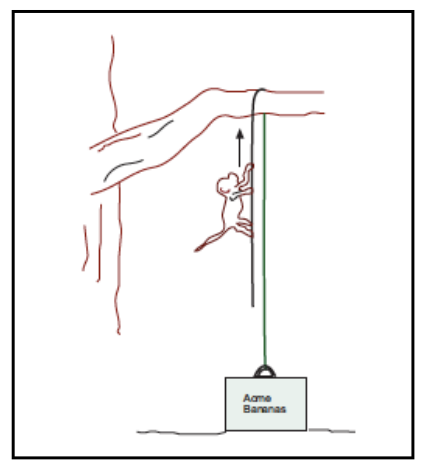
\includegraphics[clip,width = .5\columnwidth]{2bf12}
\end{center}
\end{figure}

\eje [5.3] Se tienen dos bloques de masas m = 16.0 kg y M = 88.0 kg que no están pegados. Además El
coeficiente de fricción estática entre los mismos es de 0.38, pero la superficie por debajo de M no
ofrece fricción. Entonces, ¿cuál es la mínima magnitud de la fuerza horizontal \b F requerida para
mantener a m contra M?

\begin{figure}[H]
\begin{center}
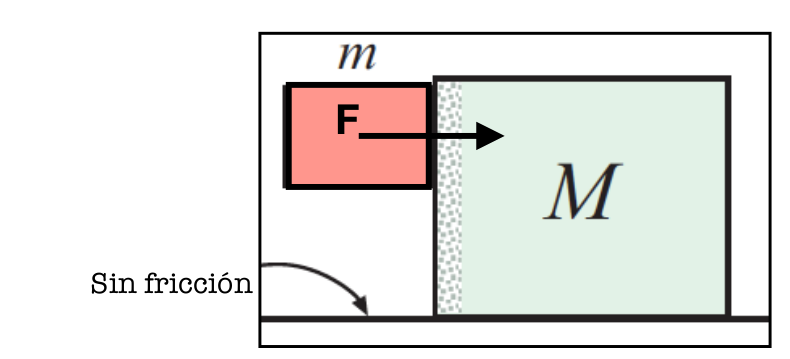
\includegraphics[clip,width = .45\columnwidth]{2bf13}
\end{center}
\end{figure}

\eje [5.5] Un bloque de 3.0 kg parte del reposo desde la cima de un plano inclinado a 30°, y se desliza
2.0 m hacia abajo en 1.5 s.

a) Encuentre la magnitud de la aceleración del bloque;

b) el coeficiente de fricción cinética entre el bloque y el plano;

c) la fuerza de fricción que actúa sobre el bloque y

d) la velocidad del bloque luego de haber recorrido 2.0 m.
\begin{figure}[H]
\begin{center}
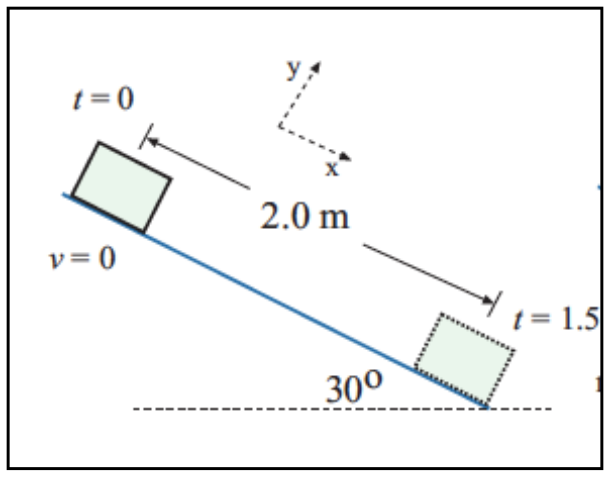
\includegraphics[clip,width = .45\columnwidth]{2bf14}
\end{center}
\end{figure}

\eje [5.8] Un bloque de 2.0 kg se coloca encima de otro de 5.0 kg como muestra la figura adjunta. El coeficiente
de fricción cinética entre el segundo bloque y la superficie es de 0.20. Una fuerza horizontal \b F se
aplica al bloque de 5.0 kg.

a) ¿Qué fuerza acelera al bloque de 2.0 kg?

b) Calcule la magnitud de la fuerza necesaria para tirar de ambos bloques hacia la derecha con
una aceleración de 3.0 m/s2;

c) encuentre el coeficiente de fricción estática mínimo entre los bloques tal que el bloque de 2.0
kg no se resbale bajo la aceleración del punto anterior.
\begin{figure}[H]
\begin{center}
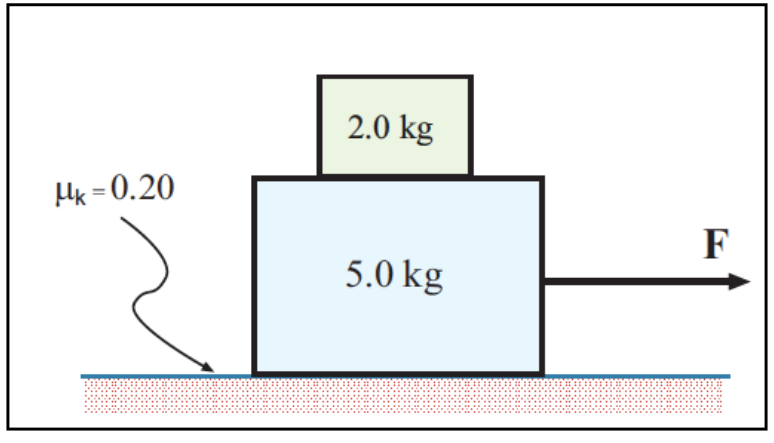
\includegraphics[clip,width = .45\columnwidth]{2bf15}
\end{center}
\end{figure}

\eje [5.10] Una masa “m" sobre una mesa sin fricción está agarrada a otra masa “M" que se encuentra
colgando, a partir de una cuerda que pasa por un agujero en el centro de la mesa. Encuentre la
velocidad a la que debe moverse la masa sobre la mesa para que la otra masa que se encuentra
colgando se mantenga en reposo.

\begin{figure}[H]
\begin{center}
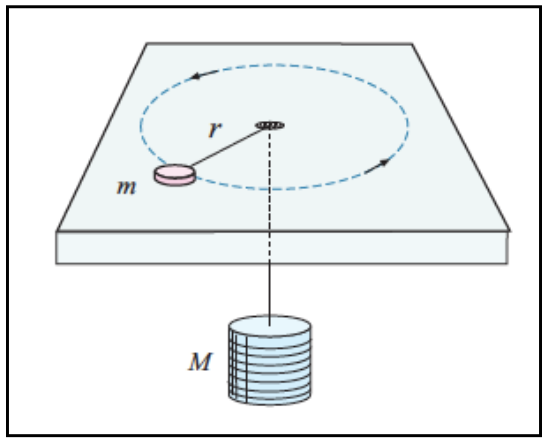
\includegraphics[clip,width = .45\columnwidth]{2bf16}
\end{center}
\end{figure}

\eje [5.12] Una moneda se apoya a 30.0 cm del centro de una mesa horizontal rotatoria, y la primera
se termina deslizando sobre la mesa cuando esta alcanza una velocidad de 50.0 cm/s.

a) ¿Qué produce la fuerza central cuando la moneda se encuentra en reposo respecto de la mesa
giratoria?

b) ¿Cuál es el coeficiente de fricción estática entre la moneda y la mesa?

\eje A continuación, otro problema cuyo nivel es elevado, si lo hacen no tienen de qué preocuparse en las instancias de
evaluación durante la cursada.

[CONCEPTUAL] Un bloque de forma de rectangular de masa 2M, se corta en dos mitades a lo largo
de la diagonal de una de las caras y de sección triangular de catetos b y c (al responder las
siguientes preguntas describa, primero, conceptualmente cómo lo irá resolviendo enunciando los
conceptos claves involucrados en su resolución).

a) Si no hay rozamiento entre las dos mitades ni con el suelo, calcular la fuerza horizontal que
hay que aplicar al de arriba para que el conjunto se mueva sin resbalar una mitad sobre la
otra, la aceleración del conjunto, y la fuerza que ejerce una mitad sobre la otra. Lo mismo si la
fuerza se aplica al de abajo y dirigida hacia la izquierda.

b) Si hay un coeficiente de roce estático $\mu_{e,A}$ entre las dos mitades, pero no en el suelo,
calcular la fuerza máxima y mínima que se puede aplicar para que una mitad no resbale sobre
la otra.

c) Lo mismo que el inciso anterior si hay un coeficiente de roce estático $\mu_{e,S}$ con el suelo,
pero no entre las dos mitades.

\end{document}